\documentclass{report}

\usepackage[ngerman]{babel}
\usepackage[utf8]{inputenc}
\usepackage[T1]{fontenc}
\usepackage{hyperref}
\usepackage{csquotes}
\usepackage[a4paper]{geometry}
\usepackage{graphicx} %Um externe Bilddateien einfügen zu können.
\usepackage{float}
\usepackage{caption}

\usepackage[
    backend=biber,
    style=apa,
    sortlocale=de_DE,
    natbib=true,
    url=false,
    doi=false,
    sortcites=true,
    sorting=nyt,
    isbn=false,
    hyperref=true,
    backref=false,
    giveninits=false,
    eprint=false]{biblatex}
\addbibresource{../references/bibliography.bib}


\title{Ethik im Umgang mit Daten}
\author{Yeva Skotar}
\date{\today}


\begin{document}

\maketitle

\abstract{
    Dies ist eine Vorlage für eine Maturarbeit in der Informatik am Gymnasium Muttenz. Sie dient dazu, die Arbeit schnell und einfach zu starten und sollte einen guten Überblick über die Arbeit bieten.
}

\tableofcontents

\chapter{Einleitung}
Unsere Welt ist mit verschiedenen Daten überquert. Die Informationsquellen können eine Enzeklopedie, 
ein Menu im Restaurant, Werbung auf den Strassen oder Google sein. Täglich sind wir am Daten Suchen, 
und es ist uns fast unmöglich die Rescherschen zu beenden, weil wir immer etwas neues, bisher noch unbekanntes 
begegnen und ein wenig Informationen darüber zu bekommen wollen. Deswegen sind die Daten ein wichtiger
Bestandteil für uns in fast allen Bereichen von unseren Leben und wir streben nach Möglichkeit,
die uns notwendige Daten so schnell wie möglich zu bekommen und aber die Qalität von den Informationen
soll immernoch hoch sein. Schon haben die gescheidene Menschen Künstliche Inteligenz entwikelt 
und damit kann die Menschheit in wenigen Sekunden allerleie Fragen beantworten haben, ohne auf ihre
Fragestellung zu achten im Gegensatz zu Suchmaschienen. Toll oder? Aber was wenn die Menschheit wird 
sich so sehr sich auf KI verlassen dass es zu einzige Datenquelle wird, wegen ihrer einfacher
Benützungsweisse? Mit der jetziger Tendenz KI zu verwenden ist es nicht ausgeschlossen.
ChatGPT und andere KI-tools ähneln sich auf einen Gesprächspartner bei der Beantwortung auf die Fragen,
deswegen heissen sie Künstliche Inteligenz - tools,aber ob die Informationen stimmen können sie nicht 
nachweisen und haben keine Verantwortung dafür. 

Es ist den Menschen überlassen ob sie die Daten überprüfen oder nicht. Wie viel Prozent 
von Leuten nach der Anfrage bei KI, dann zusätzlich noch recherschieren ob es um die aktuelle, 
wahre Informationen handelt? Daten sind nicht nur das Wissen aber auch ein entscheidener Faktor von 
unserem Verhalten während wir Entscheidungen treffen müssen. Je mehr Informationen wir verfügen
desto mehr Möglichkeiten für die Lösung unserer Problemen haben wir und es bezieht sich praktisch
auf alle Lebensbereichen, uns fehlt der Entschied zwar manchmal schwieriger als wenn die Auswahl 
von unseren Möglichkeiten reduziert ist aber je weniger wissen wir desto begrenzter sind unsere Handlungen.
Das kann dazu führen das zwischen uns bekannten Möglichkeiten uns gar keine passt. 




\chapter{Was ist KI und welche Daten besitzt die sie?}

Künstliche Intelligenz ist die Fähigkeit einer Maschine, menschliche Fähigkeiten wie logisches Denken, 
Lernen, Planen und Kreativität zu \textit{imitieren}. Die Imitation ist nicht nur in den Fähigkeiten sondern auch in den 
Funktionsweisse von KI und ihren Aufbau. Analog zu menschlichen Gehirn besitzt die KI künstlichen neuronallen Netzen und 
deren Verknüpfungen - Synapsen. Jeder KI Entwickler gibt ihr Trainingsdaten sind als Rohstoff für KI-Systeme. Die Daten sind sorgfältig 
kuratierte und bereinigte Informationen, die zu Trainingszwecken in ein System eingespeist werden.
Die anderen Daten, die KI benutzt können aus vielfältigen Quellen stammen, einschließlich Internet, Sensoren,
  Unternehmensdatenbanken und öffentlichen Datensätzen. Das bedeutet, die Daten, die KI verwendet sind genau so zuverlässig wie die Quellen aus dennen sie stammen.
KI kann aber nicht auf Daten aus dem Internet verzichten.  


bILD\begin{figure}[h]
  \centering 
  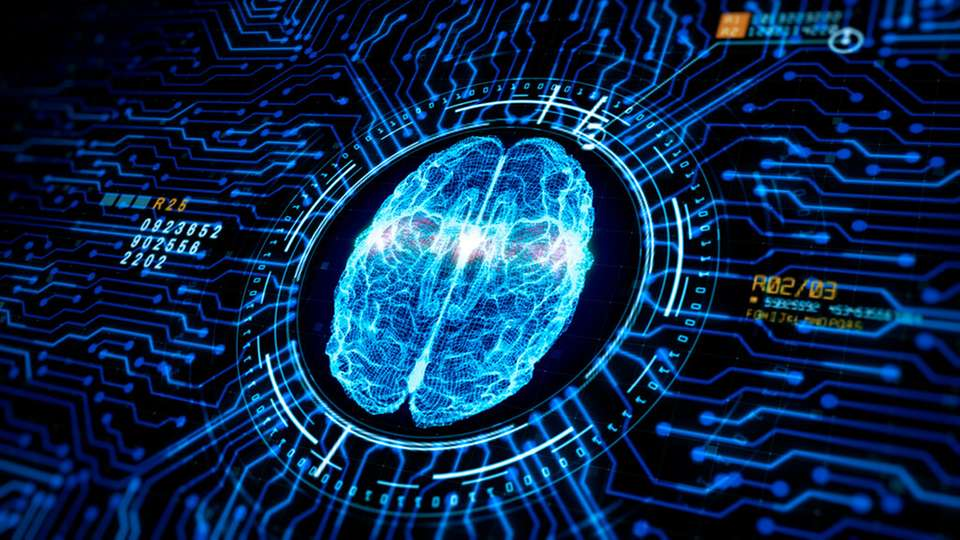
\includegraphics[width=0.5\textwidth]{ki-im-sensor.jpg} 
  \caption{Ein erstes Bild}
  \label{fig:meme}
  \end{figure}

   \chapter{Bestandteile einer KI}
 
KI-Systeme sind in der Lage, ihr Handeln anzupassen, indem sie die Folgen früherer Aktionen analysieren und autonom arbeiten.
 Generell wird das intelligente Verhalten der 
Technologien mit Mitteln der Informatik und Mathematik/Statistik simuliert.
 Die Computer werden für bestimmte Aufgaben trainiert, häufig indem sie große Datenmengen - \textit{Big data}
 verarbeiten und darin Muster erkennen. Üblicherweise entsteht eine KI durch eine Kombination aus  \textbf{Machine
  Learning} und  \textbf{Deep Learning}, zwei Subkategorien der Künstlichen Intelligenz.

 BILD2 \begin{figure}[h]
    \centering 
    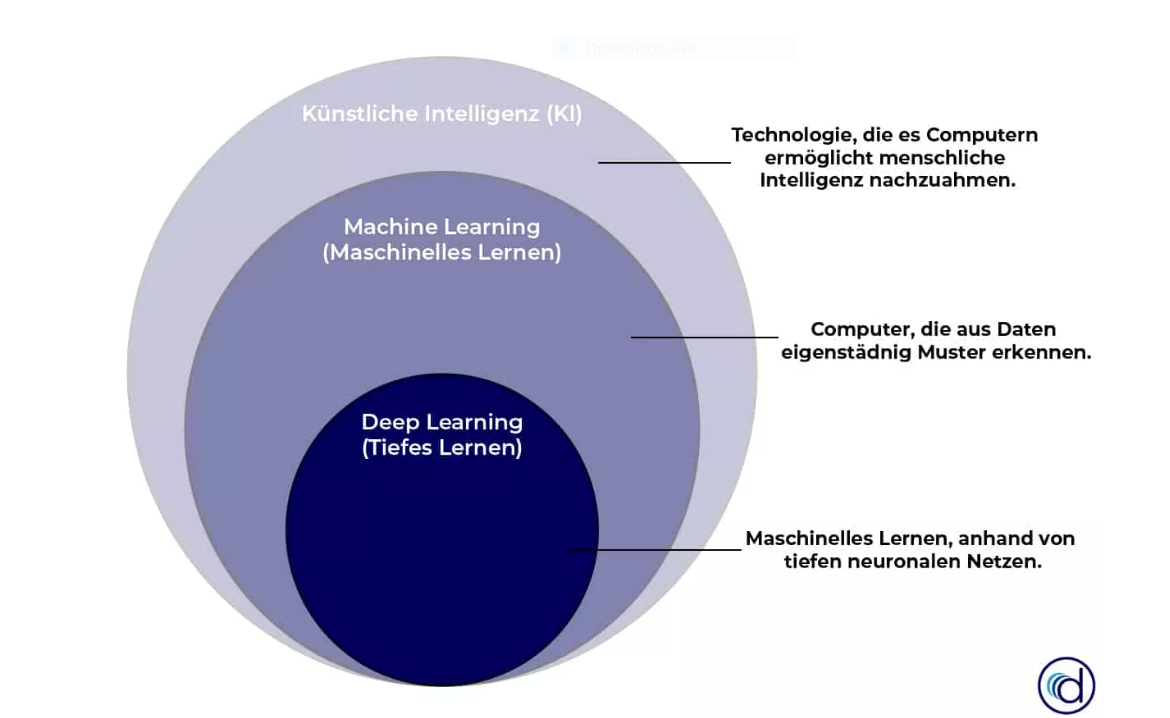
\includegraphics[width=0.8\textwidth]{ki-bestandtt.png} 
    \caption{Ein erstes Bild}
    \end{figure}

 \section{Machine Learning}
 Machine Learning ist ein Teilbereich der künstlichen Intelligenz, der Systeme in die Lage versetzt, automatisch 
 aus Erfahrungen (Daten) zu lernen und sich zu verbessern, ohne explizit programmiert zu sein.
 Maschinelles Lernen kann \textit{automatisiert Wissen generieren}, Algorithmen trainieren, Zusammenhänge identifizieren und unbekannte Muster erkennen. 
 Diese identifizierten Muster und Zusammenhänge lassen sich auf einem neuen, unbekannten Datensatz anwenden, 
 um so Vorhersagen zu treffen und Prozesse zu \textit{optimieren}.
 
 \section{Neuronale Netze}
 Ein Untergebiet von maschinellem Lernen sind neuronale Netze. Künstliche neuronale Netze bestehen aus mehreren Reihen von Datenknoten, 
 die mit gewichteten Verbindungen untereinander vernetzt sind.
 Das neuronale Netz wird trainiert, indem ihm immer wieder Daten vorgelegt werden. Durch diese Wiederholung lernt
 das neuronale Netz die Daten jedes Mal exakter einzuordnen. Das funktioniert, indem die Verbindungen
 zwischen den Neuronen-Schichten immer wieder angepasst werden. Das in den Lerndurchläufen 
 erzeugte Modell kann dann auch auf Daten angewandt werden, die die Künstliche Intelligenz im Training noch nicht kennengelernt hat.
 
 
 \section{Deep Learning} 
 Deep Learning ist eine spezielle Methode zur Informationsverarbeitung und ein Teilbereich von Machine Learning und Künstlicher 
 Intelligenz. Deep Learning analysiert großen Datensätze mit der Hilfe von neuronalen Netze. Diese von Deep Learning angewandte Funktionsweise
 agiert ähnlich wie das menschliche Gehirn. Dabei werden Daten zuerst extrahiert, anschließend analysiert, um im Anschluss eine 
 Schlussfolgerung bzw. Prognose zu erstellen. Innerhalb der Praxis wird Deep Learning hauptsächlich zum Erkennen von Bildern,
 dem Verständnis von Texten oder zur besseren Entscheidungsfindung genutzt. 
 
 \textbf{}
\textit{}
   
   \chapter{Ethische Probleme im Bezug auf KI}
   \section{ChatGPT} 
   Im November 2022 wurde den Chat GPT veröfentlicht. Viele Menschen benützen den Chat GPT alltagsmässig. Wie wurde in Kapitel
    "Was ist KI und welche Daten besitzt die sie?" erwähnt, solche Boten garantieren keine zuverlässigkeit auf die Inhalte 
    die es herausgibt. Ausserdem Menschen müssen gar es nachprüfen, sie sind oft mit den Informationen zufrieden weil es einfacher ist.
    Menschen werden weniger aufmerksam auf das was sie glauben und annehmen Iformationen uas KI tools als Wahr ohne nachzufragen.
    Ich sehe es als kein normales Verhalten, vorallem weil wir uns ständig entwickeln können in dem wir nachfragen und selber denken 
    aber mir scheint dass mit der Entwiklung der KI beginnt die Degradierung der Menschheit. 
    
    \section {Verbreitung von Vorurteilen}
    Neben den häufig ungenauer oder gar falschen aussagen können KI tools die falsche Informationen verbreiten. Die Daten die  
    Generative KI-Systeme verbrauchen können in sich Vorurteile enthalten. 
    Zusätzliche Ungenauigkeiten können durch Influencer oder die KI-Systeme selbst verstärkt werden.
    "Die Genauigkeit eines generativen KI-Systems hängt von dem verwendeten Datenkorpus und dessen Herkunft ab",
    erklärt Scott Zoldi, Chief Analytics Officer beim Kreditbewertungsunternehmen FICO. „ChatGPT-4 durchsucht das 
    Internet nach Daten, und viele davon sind wirklich Müll, was ein grundlegendes Genauigkeitsproblem bei Antworten auf Fragen 
    darstellt, auf die wir die Antwort nicht kennen.
  
   \section{Empfehlungsdienste}
   E-Shops wie Amazon oder Dienste wie Spotify oder Netflix bieten uns Empfehlungssysteme, die relevanten Inhalte
    aus einem überwältigenden Angebot zu finden helfen. Sie steuern aber auch die Neuigkeiten und Gruppen,
 die uns in sozialen Medien vorgeschlagen. Bei solchen Vorschlagen basieren die KI Algorythmen auf die Anfregen die wir vorher gemacht haben
 und so ist die Chanse dass wir auf etwas Neues für uns bei Resherschen zustossen ist gering. Wir werden nur das 
 sehen was wir schon kennen und es wird uns nicht nur langweilen mit der Zeit aber auch verhindern von Entdekungen von 
 neuen Interessen. Somit kann man wieder die Bremsung von unsere Entwiklung hervornehmen.



 \section{Scamming}
 Seit Ende März 2023 gestattet OpenAI die Integration von ChatGPT in die Produkte von Unternehmen, 
 die ihr Angebot online präsentieren, zum Beispiel in Form virtueller Assistenten, die Termine speichern. 
 Dieser Mechanismus macht den Chatbot verwundbar, vor allem für die sogenannte „indirekte Eingabeaufforderung“.
 Dabei nehmen Dritte Änderungen an einer Website vor, indem sie versteckten Text hinzufügen. Dieser sorgt dafür,
dass die KI anders agiert als vorgesehen und so etwa sensible Daten von Nutzer:innen abfragt. Kriminelle nutzen 
zum Beispiel vermehrt Social Media und E-Mail, um User:innen auf Websites mit solchen verborgenen Eingabeaufforderungen zu locken.
Daraus lässt sich schliessen, Menschen die KI benützen und dazu ihr steuern können, können es für eigene Zwecke mit Schaden 
für die anderen Benützer anwenden. 

 Wie wir es schon wissen benützt die KI alle öffentliche Internetresoursen und bearbeitet sie. Das können auch unsere Fotos, Videos 
 die mal irgendwo im Netz aufgetaucht waren, vielleicht  Blogs von Menschen aller Berufen und Nationalitäten. 
Ist das nicht gefährlich wenn KI unsere Daten ins spiel nehmen beginnt? Natürlich weisst fast jeder das man gut nachdenken 
muss bevor man irgendwelche Informationen ins Netz lädt und trotzdem gibt es genug von solchen die 


\section{Rolle der Mitarbeiter}
  KI kann einen Großteil der täglichen Aufgaben von Wissensarbeitern übernehmen, darunter Schreiben,
   Codieren, Erstellen von Inhalten, Zusammenfassen und Analysieren.  Jedes Jahr es werden immer weniger Leute auf den
   Betrieben und Fabriken angestellt und das ständige weiterentwicklung von KI-Systemen führt dazu das es irgendwann gar keine Menschen
 für die Wirtschaftssystheme braucht. Sowas wäre aber idel für die Cheffs die das Markt kontrolieren, sie würden keine Löhne bezahlen müssen 
 nur ein Mal kauffen die Maschine die die Arbeit macht und kann grösstwahrscheinlich mehr als ein Mensch dienen, sie wird nicht kank und braucht keine 
 Ferien. 

\textbf{}
\textit{}
   \capter{Fazit}




\input{chap_methode.tex}

\section{Quellen}
\parskip = 1em %Abstand
\parindent = 0em %Einrückung


\begin{itemize}
\item \url{https://www.produktion.de/technik/zukunftstechnologien/kuenstliche-intelligenz/kuenstliche-intelligenz-verstaendlich-erklaert-243.html#wie-funktioniert-kuenstliche-intelligenz}
\item \url{https://www.europarl.europa.eu/topics/de/article/20200827STO85804/was-ist-kunstliche-intelligenz-und-wie-wird-sie-genutzt}
\item \url{https://digitalzentrum-augsburg.de/kuenstliche-intelligenz-einfach-erklaert/}
\item \url{https://datasolut.com/anwendungsgebiete-von-kuenstlicher-intelligenz/} -- 2Bild
\item \url{https://datasolut.com/was-ist-deep-learning/} 
\item \url{https://digital-zentral.de/die-datenquelle-der-kuenstlichen-intelligenz-woher-bezieht-eine-ki-ihre-informationen/}
\item \url{https://datasolut.com/neuronale-netzwerke-einfuehrung/#definition-neuronales-netz}
\item \url{https://www.iks.fraunhofer.de/de/themen/kuenstliche-intelligenz.html}
\item \url{https://datasolut.com/anwendungsgebiete-von-kuenstlicher-intelligenz/#Was_ist_kuenstliche_Intelligenz}
\item \url{https://www.computerweekly.com/de/tipp/Die-8-groessten-ethischen-Bedenken-beim-Einsatz-generativer-KI}
\end{itemize}

\printbibliography

\end{document}
